%% Application à des données réelles
% le Sweaveopt


\section{Application à des données réelles}

\subsection{Analyse de données}



\begin{frame}{Analyse de données}
Pour mettre en application l'approche proposée par \cite{chavez2016extreme}, deux jeux de données du paquetage \texttt{CASdatasets} sont utilisés. Soit \texttt{auscathist} et \texttt{nzcathist}. \\~\\

Ces données représentent respectivement l'historique des catastrophes naturelles pour l'Australie ainsi que pour la Nouvelle-Zélande. Les prochaines diapositives présentent une analyse globale des données utilisées.
\end{frame}


\begin{frame}
\begin{figure}
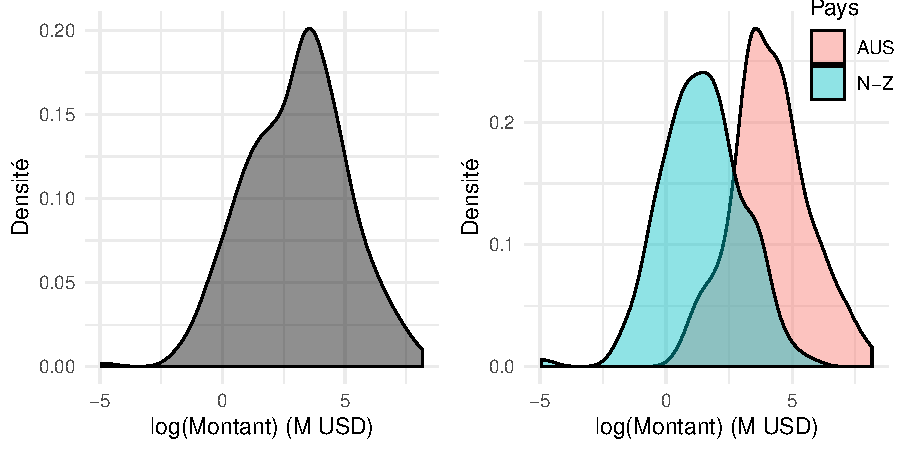
\includegraphics[width=.8\textwidth]{images/fig-005.pdf}
\caption{Densité du logarithme du montant des catastrophes}
\end{figure}
\end{frame}

\begin{frame}
\begin{figure}
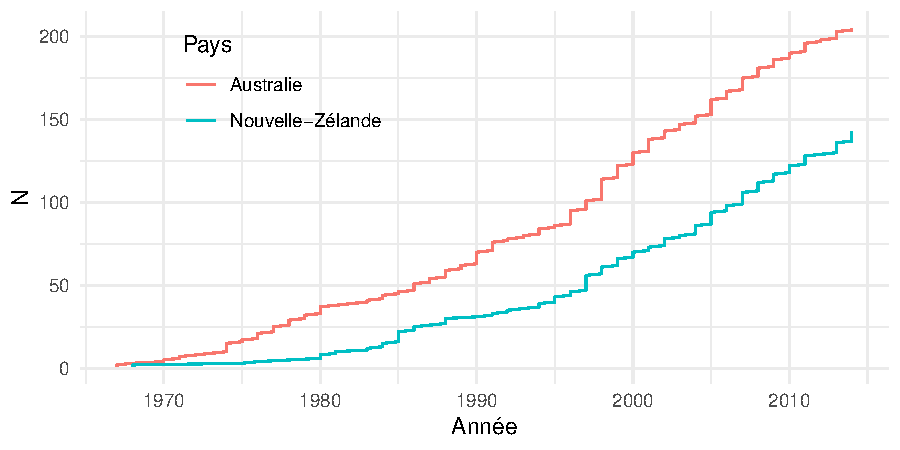
\includegraphics[width=.8\textwidth]{images/fig-006.pdf}
\caption{Nombre cumulatif de catastrophes par pays}
\end{figure}
\end{frame}

\begin{frame}
\begin{figure}
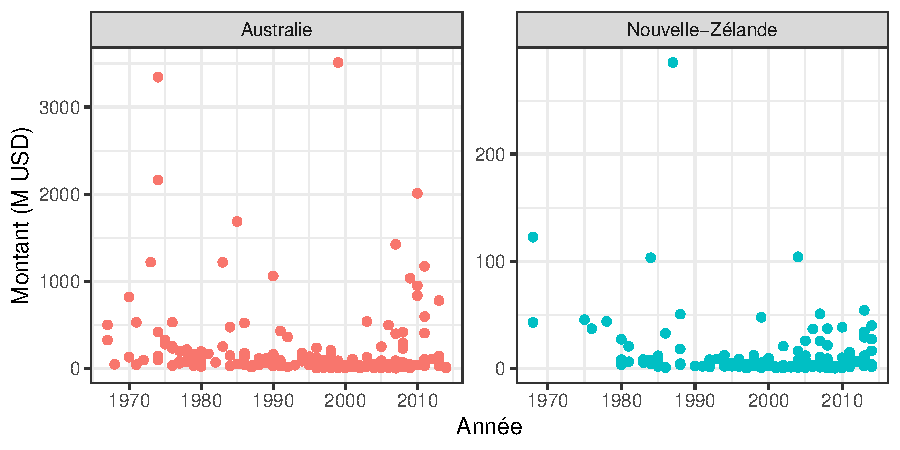
\includegraphics[width=.8\textwidth]{images/fig-007.pdf}
\caption{Évolution des catastrophes par pays}
\end{figure}
\end{frame}

\begin{frame}
% latex table generated in R 3.6.1 by xtable 1.8-4 package
% Mon Nov 25 16:50:46 2019
\begin{table}[ht]
\centering
\begin{tabular}{cccccccc}
  \hline
Type & N & Moyenne & Écart & Minimum & Médiane & Q3 & Maximum \\ 
  \hline
Bushfire & 26 & 143 & 259 & 7 & 39 & 134 & 1217 \\ 
  Cyclone & 37 & 325 & 675 & 2 & 88 & 217 & 3343 \\ 
  Earthquake & 9 & 56 & 91 & 0 & 25 & 47 & 286 \\ 
  Flood & 83 & 62 & 230 & 0 & 5 & 39 & 2010 \\ 
  Flood, Storm & 36 & 54 & 79 & 1 & 24 & 71 & 414 \\ 
  Hailstorm & 41 & 274 & 606 & 0 & 75 & 235 & 3511 \\ 
  Other & 12 & 121 & 296 & 2 & 6 & 50 & 1035 \\ 
  Power outage & 2 & 6 & 6 & 1 & 6 & 8 & 11 \\ 
  Storm & 86 & 97 & 228 & 0 & 28 & 57 & 1424 \\ 
  Tornado & 12 & 7 & 13 & 0 & 3 & 7 & 47 \\ 
  Weather & 4 & 11 & 11 & 2 & 6 & 13 & 27 \\ 
   \hline
\end{tabular}
\caption{Résumé statistique des montants (M USD) de catastrophes par Type} 
\label{tab:3.6}
\end{table}\end{frame}

\subsection{Approche classique}

\begin{frame}
\begin{itemize}
\item Par souci de manque de temps, les résultats obtenus avec l'approche classique ne seront pas montrés de façon détaillée. On conlut que cette approche n'est pas tout à fait adéquate dans le cas présent. 
\item Cette approche reste viable, rapide et peut être une bonne solution lorsque seulement les montants sont disponibles.
\item Un seuil de 10 M USD fut sélectionné
\end{itemize}
\end{frame}



\subsection{Approche dynamique à deux variables}

\subsection{Approche dynamique à trois variables}
